\documentclass[a4paper,12pt,oneside, tikz]{book}  
\usepackage[utf8]{inputenc}
\usepackage{tcolorbox}
\usepackage{amsmath,amssymb,amsthm, enumitem, hyperref, tabto} 
\usepackage[T1]{fontenc}
\usepackage[utf8]{inputenc}
\usepackage[english]{babel}
\usepackage{wrapfig}
\usepackage{lastpage}
\usepackage{tikz}
\usetikzlibrary{external}
\tikzexternalize % activate!
\usepackage[american]{circuitikz}
\usepackage[absolute,overlay]{textpos}
\usepackage[left=2cm,right=2cm]{geometry}
\usepackage[english]{babel}
\usepackage{fancyhdr}
\usepackage{float}
\hypersetup{
    colorlinks=true,
    linkcolor=blue,
    filecolor=magenta,      
    urlcolor=cyan,
    pdftitle={Studio 4},
    pdfpagemode=FullScreen,
    }

\urlstyle{same}
\usepackage{xcolor}
\usepackage{colortbl}

\usepackage{graphicx, multicol, latexsym}
\usepackage{blindtext}
\usepackage{subfigure}
\usepackage{caption}
\usepackage{capt-of}
\usepackage{tabu}
\usepackage{booktabs}

\usepackage{fancyhdr}            % Permits header customization. See header section below.
\fancypagestyle{plain}{
    \lhead{}
    \fancyhead[R]{\thepage}
    \fancyhead[L]{}
    \renewcommand{\headrulewidth}{0pt}
    \fancyfoot{}
}

\pagestyle{fancy}
\fancyhead[R]{\thepage}
\fancyhead[L]{}
\renewcommand{\headrulewidth}{0pt}
\fancyfoot{}

\usepackage{array}
\newcolumntype{P}[1]{>{\centering\arraybackslash}p{#1}}

\usepackage{titlesec}

\titleformat{\chapter}[display]{\normalfont\huge\bfseries}{\chaptertitlename\ \thechapter}{20pt}{\Huge}

% this alters "before" spacing (the second length argument) to 0
\titlespacing*{\chapter}{0pt}{0pt}{40pt}


\addto\captionsenglish{\renewcommand{\chaptername}{Activity}} 


\title{\textbf{Comparators and LPFs} Studio Report \\ CG1111A Studio 9}

\author{Prannaya Gupta (B02)}

\begin{document}

\maketitle

\chapter{Non-inverting Comparator}

\section{Preparation}

\begin{table}[H]
    \centering
    \begin{tabular}{|c|c|c|c|}
        \hline S/N & $V_\text{in}$ (V) & $V_\text{ref}$ (V) & $V_\text{out}$ (V)  \\
        \hline 1 & +2.5 & 0 & 5 \\
            2 & +3.5 & +3.75 & 0 \\
            3 & +1.25 & -0.5 & 5 \\
            4 & -3 & -1 & 0 \\
            5 & -2.5 & +2.5 & 0 \\
        \hline
    \end{tabular}
    \caption{Theoretical Values for $V_\text{out}$}
    \label{tab:vout1}
\end{table}

\begin{tcolorbox}
\textbf{How would the output voltage values change if a dual power supply of +5V and –5V is provided to the op amp?} \\
Those with $V_\text{out} = 0$ V would instead have $V_\text{out} = -5$ V instead, assuming no overhead.
\end{tcolorbox}

\section{Experimental Data}

\begin{figure}[H]
    \centering
    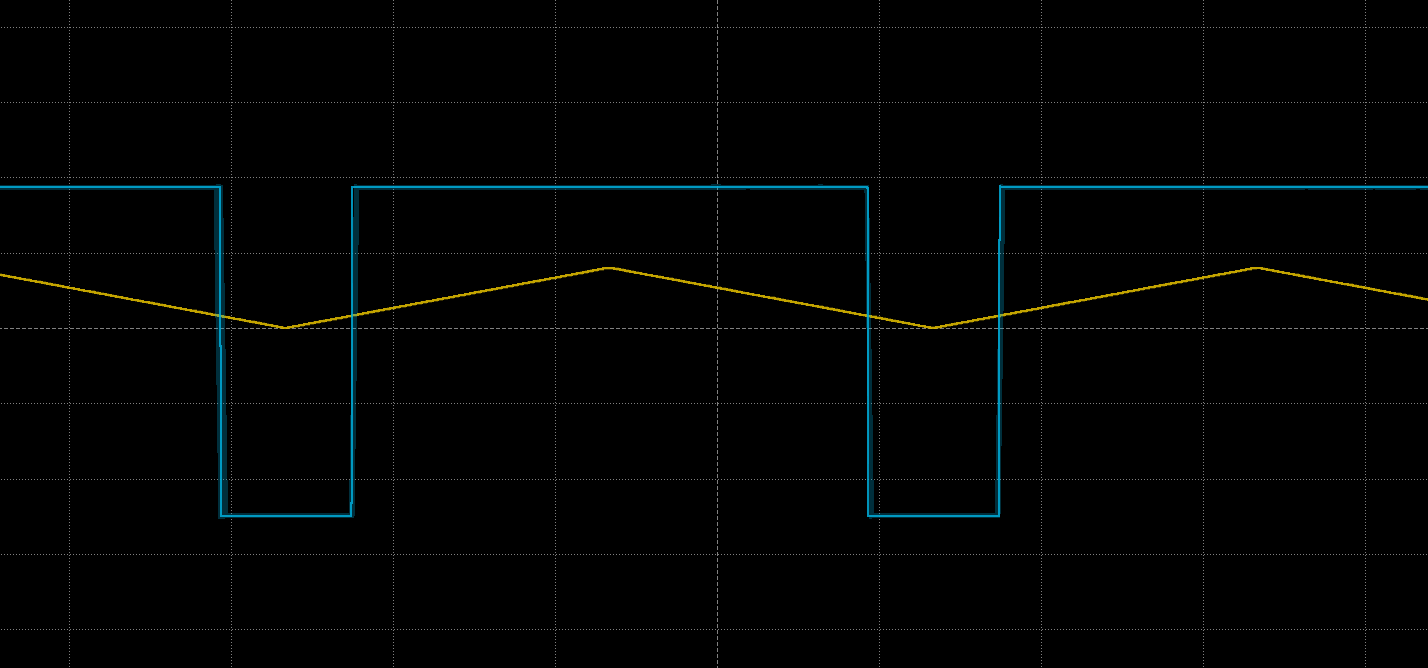
\includegraphics[width=0.8\textwidth]{./images/0_7.png}
    \caption{$V_\text{ref} = 0.7$ V}
    \label{fig:0_7}
\end{figure}

\begin{figure}[H]
    \centering
    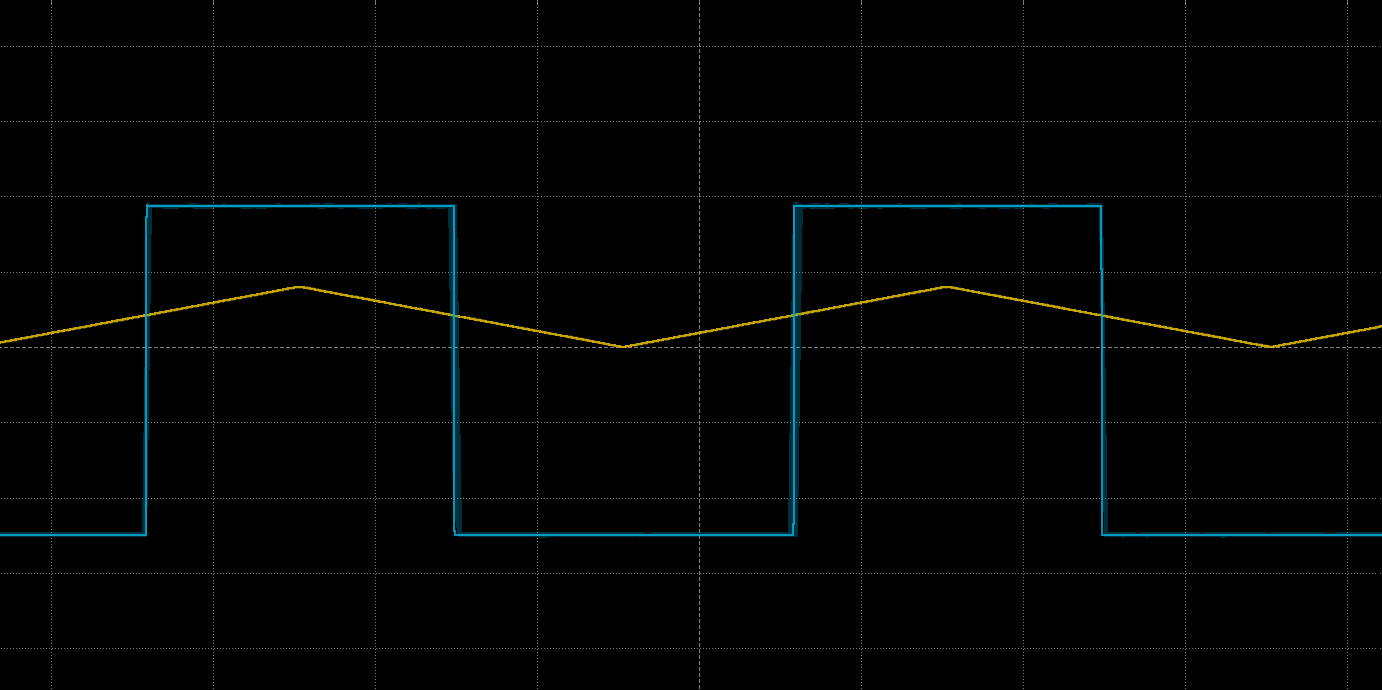
\includegraphics[width=0.8\textwidth]{./images/2_0.png}
    \caption{$V_\text{ref} = 2.0$ V}
    \label{fig:0_7}
\end{figure}

\begin{figure}[H]
    \centering
    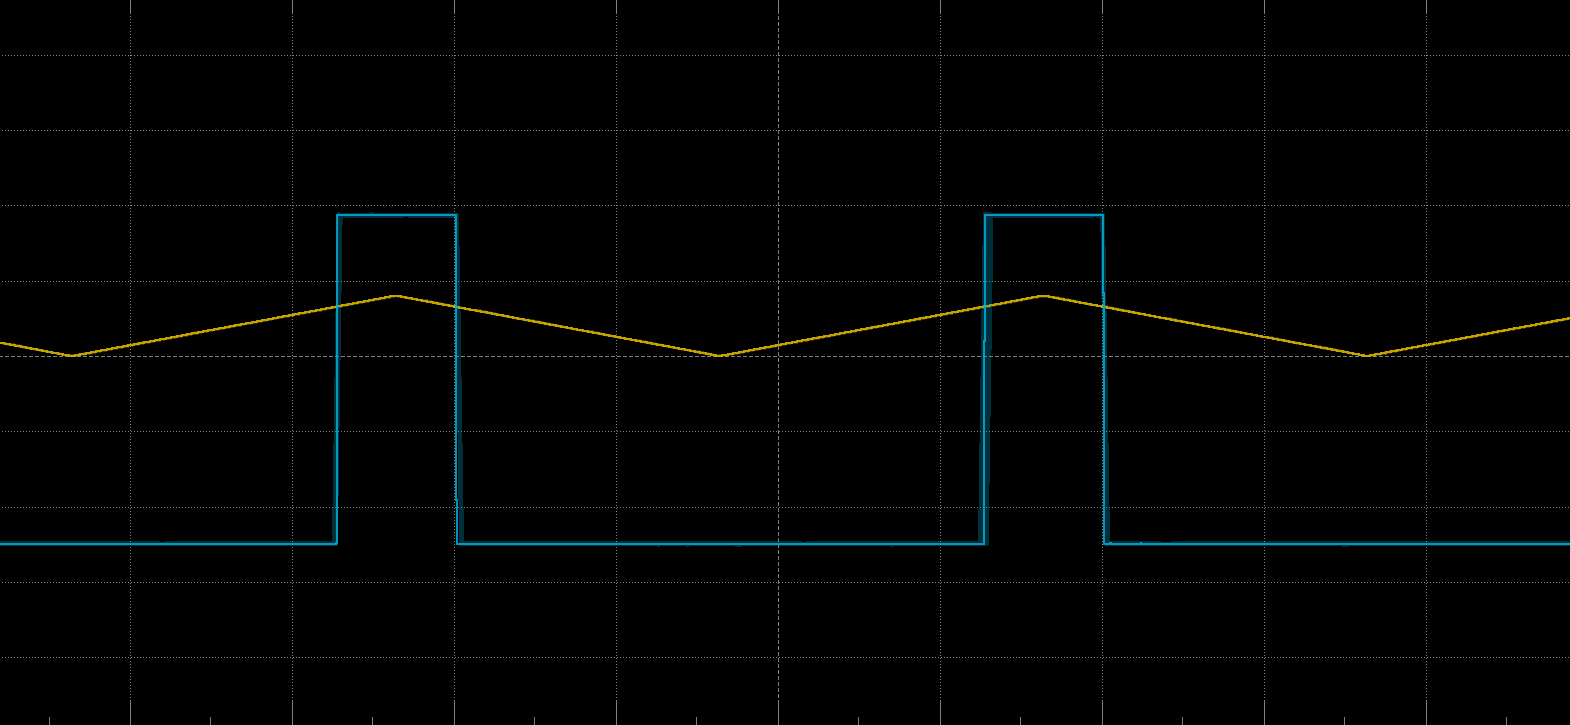
\includegraphics[width=0.8\textwidth]{./images/3_2.png}
    \caption{$V_\text{ref} = 3.2$ V}
    \label{fig:0_7}
\end{figure}

\begin{tcolorbox}
\textbf{What type of waveform do you observe at the output? Does it tally with your expectation for the output? How does the output waveform vary with the change in the reference voltage? Explain. } \\
We see a square wave that toggles between a higher value (+5) and a smaller value (-5) as the triangular waveform from the AD2 enters specific higher voltages. This is expectant as the waveform slowly exceeds and goes below the referential value $V_\text{ref}$. This means that as it enter certain ranges, the voltage toggles between 5 V and -5 V.

\end{tcolorbox}

\chapter{Active Low-Pass Filter}
\begin{tcolorbox}
\textbf{What is the voltage gain expression ($V_\text{out}/V^+$) for this op amp circuit? Calculate the value of the gain given the resistance values. }\\
$$V_\text{out}/V^+ = 1 + \frac{R_f}{R_\text{in}}$$

\end{tcolorbox}

The experimental value for $R$ is \textbf{390} k$\Omega$.

\begin{table}[H]
    \centering
    \begin{tabular}{|c|c|c|c|c|c|}
        \hline S/N & Frequency (Hz) & $V_\text{in}$ (V) & $V_\text{out}$ (V) & Gain ($V_\text{out}/V_\text{in}$) & Gain in dB \\
        \hline 1 & 200 & 3.2138 & 6.4807 & 2.0165 & 6.0921 \\
        \hline 2 & 500 & 3.2271 & 6.4143 & 
        1.9876 & 5.9667 \\
        \hline 3 & 1000 & 3.2138 & 6.255 & 1.9463 & 5.7842 \\
        \hline 4 & 1500 & 3.2138 & 6.0558 & 1.8843 & 5.5031 \\
        \hline 5 & 2000 & 3.2404 & 5.7902 & 1.7869 & 5.0419  \\
        \hline 6 & 3000 & 3.2537 & 5.1926 & 1.5959 & 4.0601 \\
        \hline 7 & 5000 & 3.2537 & 4.0637 & 1.2489 & 1.9309 \\
        \hline 8 & 10k & 3.2205 & 2.3838 & 0.7402 & -2.6131 \\
        \hline 9 & 20k & 3.2404 & 1.2483 & 0.38523 & -8.2856 \\
        \hline 10 & 50k & 3.2404 & 0.55113 & 0.17008 & -15.387 \\
        \hline
    \end{tabular}
    \caption{Experimental Readings}
    \label{tab:exp}
\end{table}

\begin{figure}[H]
    \centering
    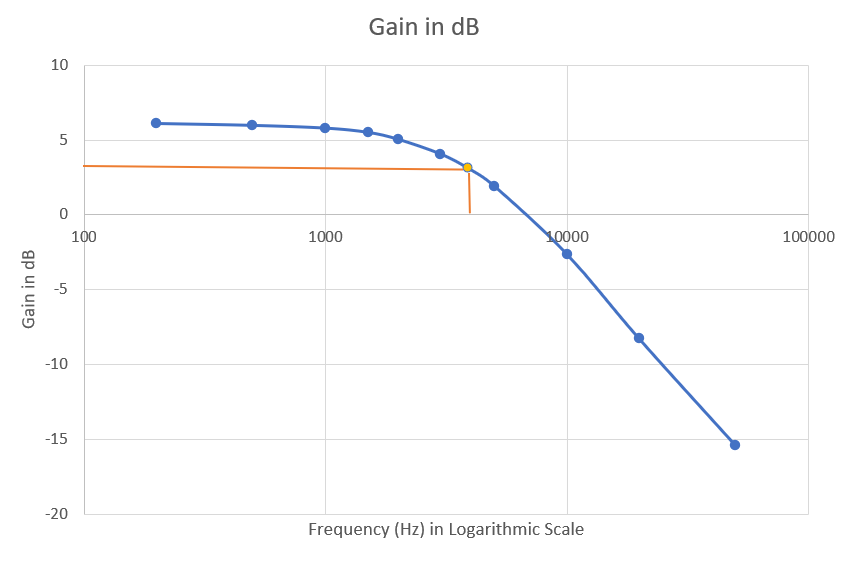
\includegraphics{./images/gain.png}
    \caption{Curve of Gain in dB against Freqeuncy (Hz) in Log Scale.}
    \label{fig:gain}
\end{figure}

The offset frequency occurs at 3.0921 dB gain, which occurs at $f = 3920$ Hz.

On the other hand, when computed:

$$f_\text{theory} = \frac{1}{2\pi RC} = \frac{1}{2\pi(390\times 10^3)(100 \times 10^{-9})} = 4.0809\text{ Hz}$$

This value is much smaller, and this can be largely attributed to the resistance of the wires and the breadboard which can significantly affect the results.

\begin{tcolorbox}
\textbf{What value of capacitor would you use if a cut-off frequency of about 2 kHz is required? Assume that R remains unchanged. }
$$C = \frac{1}{2\pi Rf} = \frac{1}{2\pi (390 \times 10^3)(2\times 10^3)} = 2.0404 \times 10^{-10}\text{ C}$$
\end{tcolorbox}


\end{document}